\documentclass[12pt,a4paper]{article}

% ---------------------------------------------------------
% PACKAGES
% ---------------------------------------------------------
\usepackage[a4paper,margin=1in]{geometry}
\usepackage{graphicx}
\usepackage{float}
\usepackage{amsmath}
\usepackage{amssymb}
\usepackage{booktabs}
\usepackage{array}
\usepackage{multirow}
\usepackage{enumitem}
\usepackage{xcolor}
\usepackage{hyperref}
\usepackage{caption}
\usepackage{subcaption}
\usepackage{listings}
\usepackage{fancyhdr}
\usepackage{setspace}
\usepackage{longtable}

% ---------------------------------------------------------
% HYPERLINK SETTINGS
% ---------------------------------------------------------
\hypersetup{
    colorlinks=true,
    linkcolor=blue,
    urlcolor=blue,
    citecolor=blue
}

% ---------------------------------------------------------
% CODE LISTING SETTINGS
% ---------------------------------------------------------
\definecolor{codegreen}{rgb}{0,0.5,0}
\definecolor{codegray}{rgb}{0.5,0.5,0.5}
\definecolor{codeblue}{rgb}{0,0,0.8}
\definecolor{backcolour}{rgb}{0.96,0.96,0.96}

\lstdefinestyle{pythonstyle}{
    backgroundcolor=\color{backcolour},
    commentstyle=\color{codegreen},
    keywordstyle=\color{codeblue},
    numberstyle=\tiny\color{codegray},
    stringstyle=\color{red},
    basicstyle=\ttfamily\footnotesize,
    breaklines=true,
    captionpos=b,
    keepspaces=true,
    numbers=left,
    numbersep=5pt,
    showspaces=false,
    showstringspaces=false,
    showtabs=false,
    tabsize=4,
    language=Python
}

\lstset{style=pythonstyle}

% ---------------------------------------------------------
% LINE SPACING
% ---------------------------------------------------------
\onehalfspacing

% ---------------------------------------------------------
% HEADER / FOOTER
% ---------------------------------------------------------
\pagestyle{fancy}
\fancyhf{}
\lhead{CS3807 -- Deep Learning Laboratory}
\rhead{Experiment 4}
\cfoot{\thepage}

% ---------------------------------------------------------
% DOCUMENT
% ---------------------------------------------------------
\begin{document}

% =========================================================
% TITLE PAGE
% =========================================================

\begin{titlepage}

\begin{center}

\vspace*{1cm}

{\Large \textbf{SHIV NADAR UNIVERSITY CHENNAI}}\\[0.4cm]

{\large \textbf{B.Tech Artificial Intelligence and Data Science}}\\[1.2cm]

{\Large \textbf{CS3807 -- DEEP LEARNING LABORATORY}}\\[1.2cm]

\rule{\textwidth}{1pt}\\[0.4cm]

{\LARGE \textbf{EXPERIMENT 4}}\\[0.4cm]

{\Large
\textbf{Comparative Study of Deep Convolutional Neural Network}\\
\textbf{Architectures Using Transfer Learning}
}\\[0.4cm]

\rule{\textwidth}{1pt}\\[2cm]

\begin{tabular}{ll}
\textbf{Degree} & B.Tech Artificial Intelligence and Data Science \\[0.3cm]
\textbf{Semester} & V \\[0.3cm]
\textbf{Subject Code} & CS3807 \\[0.3cm]
\textbf{Academic Year} & 2026--27 \\
\end{tabular}

\vfill

\textbf{Submitted By}\\[0.3cm]

\textbf{Name:} Ashwin S\\
\textbf{Register Number:} 24011101006\\
\textbf{Section:} A

\vfill

\textbf{Department of Artificial Intelligence and Data Science}\\
\textbf{Shiv Nadar University Chennai}

\end{center}

\end{titlepage}

% =========================================================
% TABLE OF CONTENTS
% =========================================================

\tableofcontents
\newpage

% =========================================================
% 1. OBJECTIVE
% =========================================================

\section{Objective}

The objectives of this experiment are:

\begin{enumerate}
    \item To study the evolution of deep Convolutional Neural Network (CNN) architectures.
    \item To compare LeNet-5, AlexNet, VGG16, GoogleNet, and ResNet architectures.
    \item To understand the concept of transfer learning.
    \item To implement transfer learning using a pretrained CNN model.
    \item To fine-tune selected layers of a pretrained CNN.
    \item To compare classification performance using accuracy, precision, recall, F1-score, and confusion matrix.
\end{enumerate}

% =========================================================
% 2. LEARNING OUTCOMES
% =========================================================

\section{Learning Outcomes}

After completing this experiment, the following learning outcomes were achieved:

\begin{enumerate}
    \item Modern CNN architectures were studied and analyzed.
    \item The architectural differences between LeNet, AlexNet, VGG16, GoogleNet, and ResNet were understood.
    \item Transfer learning was implemented using a pretrained ResNet50 model.
    \item Fine-tuning of the pretrained convolutional layers was performed.
    \item The trained model was evaluated using multiple classification metrics.
\end{enumerate}

% =========================================================
% 3. INTRODUCTION
% =========================================================

\section{Introduction}

Deep Convolutional Neural Networks have become one of the most successful approaches for computer vision applications. CNNs automatically learn hierarchical representations from images, starting from simple features such as edges and textures and gradually learning more complex structures such as shapes and objects.

The evolution of CNN architectures has focused on improving classification accuracy, increasing network depth, reducing computational complexity, and making the training process more stable.

The progression began with LeNet-5 and later advanced through AlexNet, VGG16, GoogleNet, and ResNet. Each architecture introduced important innovations that significantly influenced modern deep learning.

In this experiment, transfer learning is used to adapt a pretrained CNN model trained on ImageNet to the CIFAR-10 image classification task. ResNet50 is used as the primary pretrained architecture.

% =========================================================
% 4. EVOLUTION OF CNN ARCHITECTURES
% =========================================================

\section{Evolution of CNN Architectures}

\begin{table}[H]
\centering
\caption{Evolution of Major CNN Architectures}
\begin{tabular}{p{3cm}p{1.5cm}p{8cm}}
\toprule
\textbf{Architecture} & \textbf{Year} & \textbf{Major Contribution} \\
\midrule
LeNet-5 & 1998 & First successful practical convolutional neural network for handwritten digit recognition. \\
AlexNet & 2012 & Introduced ReLU activation, dropout, GPU-based training, and data augmentation. \\
VGG16 & 2014 & Demonstrated the effectiveness of deep networks using uniform $3\times3$ convolution filters. \\
GoogleNet & 2014 & Introduced the Inception module for multi-scale feature extraction. \\
ResNet & 2015 & Introduced residual learning and skip connections, enabling very deep networks. \\
\bottomrule
\end{tabular}
\end{table}

% =========================================================
% 5. LENET
% =========================================================

\section{LeNet-5}

LeNet-5 was proposed by Yann LeCun and his collaborators in 1998 for handwritten digit recognition. It consists of convolutional layers, average pooling layers, and fully connected layers.

The architecture demonstrated that convolutional networks could automatically learn useful image features without requiring handcrafted feature extraction.

\subsection{Advantages}

\begin{itemize}
    \item Small number of parameters.
    \item Fast training.
    \item Low computational complexity.
    \item Suitable for handwritten digit recognition and OCR applications.
\end{itemize}

% =========================================================
% 6. ALEXNET
% =========================================================

\section{AlexNet}

AlexNet achieved a major breakthrough in image classification by winning the ImageNet Large Scale Visual Recognition Challenge in 2012.

It introduced several techniques that became standard in deep learning.

\subsection{Major Innovations}

\begin{itemize}
    \item Rectified Linear Unit (ReLU) activation.
    \item Dropout regularization.
    \item GPU-based training.
    \item Data augmentation.
    \item Deeper CNN architecture.
\end{itemize}

The success of AlexNet demonstrated that deep neural networks trained on GPUs could achieve significantly better image classification performance than traditional computer vision approaches.

% =========================================================
% 7. VGG16
% =========================================================

\section{VGG16}

VGG16 was proposed by Simonyan and Zisserman. It uses a deep architecture consisting primarily of $3\times3$ convolutional filters.

Using multiple small filters instead of larger filters allows the network to introduce additional nonlinearities while keeping the receptive field effective.

\subsection{Advantages}

\begin{itemize}
    \item Simple and uniform architecture.
    \item Excellent feature extraction capability.
    \item High classification accuracy.
    \item Easy to understand and implement.
\end{itemize}

% =========================================================
% 8. GOOGLENET
% =========================================================

\section{GoogleNet}

GoogleNet, also known as Inception, was introduced by Szegedy et al. in 2014.

Its main contribution was the Inception module. Instead of applying only one type of convolution, an Inception module performs several operations in parallel.

These include:

\begin{itemize}
    \item $1\times1$ convolution.
    \item $3\times3$ convolution.
    \item $5\times5$ convolution.
    \item Max pooling.
\end{itemize}

The resulting feature maps are concatenated to obtain a multi-scale representation.

The $1\times1$ convolution is also used for dimensionality reduction, which reduces the number of parameters and computational cost.

% =========================================================
% 9. RESNET
% =========================================================

\section{ResNet}

Residual Network (ResNet) was introduced by He et al. to address the degradation and vanishing-gradient problems associated with very deep neural networks.

Instead of directly learning a mapping $H(x)$, ResNet learns a residual mapping:

\begin{equation}
F(x) = H(x) - x
\end{equation}

Therefore, the output of a residual block is:

\begin{equation}
H(x) = F(x) + x
\end{equation}

Here:

\begin{itemize}
    \item $F(x)$ represents the residual mapping.
    \item $x$ represents the identity mapping.
    \item $F(x)+x$ represents the final output of the residual block.
\end{itemize}

\subsection{Advantages}

\begin{itemize}
    \item Helps prevent vanishing gradients.
    \item Enables training of very deep neural networks.
    \item Improves gradient flow.
    \item Faster convergence.
    \item High classification performance.
\end{itemize}

% =========================================================
% 10. ARCHITECTURE COMPARISON
% =========================================================

\section{Comparison of CNN Architectures}

\begin{table}[H]
\centering
\caption{Comparison of Major CNN Architectures}
\begin{tabular}{lccc}
\toprule
\textbf{Architecture} & \textbf{Depth} & \textbf{Parameters} & \textbf{Main Contribution} \\
\midrule
LeNet-5 & 7 & $\sim60$K & First practical CNN \\
AlexNet & 8 & $\sim61$M & ReLU and Dropout \\
VGG16 & 16 & $\sim138$M & Deep $3\times3$ convolutions \\
GoogleNet & 22 & $\sim6.8$M & Inception modules \\
ResNet50 & 50 & $\sim25.6$M & Residual learning \\
\bottomrule
\end{tabular}
\end{table}

% =========================================================
% 11. DILATED CONVOLUTION
% =========================================================

\section{Dilated Convolution}

Dilated convolution, also called atrous convolution, increases the receptive field of a convolutional operation without proportionally increasing the number of parameters.

For a standard convolution:

\begin{equation}
D=1
\end{equation}

For a dilated convolution:

\begin{equation}
D>1
\end{equation}

where $D$ represents the dilation rate.

Dilated convolutions are widely used in:

\begin{itemize}
    \item Semantic segmentation.
    \item Medical image analysis.
    \item Satellite image processing.
    \item Object localization.
\end{itemize}

% =========================================================
% 12. TRANSPOSE CONVOLUTION
% =========================================================

\section{Transpose Convolution}

Transpose convolution is a learnable upsampling operation used to increase the spatial dimensions of feature maps.

Unlike pooling, which reduces spatial dimensions, transpose convolution increases them using learnable parameters.

Applications include:

\begin{itemize}
    \item Image super-resolution.
    \item Autoencoders.
    \item Generative Adversarial Networks.
    \item Image generation.
    \item Semantic segmentation.
\end{itemize}

% =========================================================
% 13. TRANSFER LEARNING
% =========================================================

\section{Transfer Learning}

Transfer learning uses knowledge learned by a model on a large dataset and transfers that knowledge to another task.

In this experiment, ResNet50 pretrained on ImageNet is used as the feature extractor for CIFAR-10 classification.

The transfer learning workflow is:

\begin{enumerate}
    \item Load the pretrained ResNet50 model.
    \item Remove its original ImageNet classification layer.
    \item Freeze the convolutional base.
    \item Add a Global Average Pooling layer.
    \item Add a fully connected Dense layer.
    \item Add a 10-class Softmax output layer.
    \item Train the newly added classification layers.
    \item Unfreeze selected layers and perform fine-tuning.
\end{enumerate}

\subsection{Advantages of Transfer Learning}

\begin{itemize}
    \item Faster convergence.
    \item Reduced training time.
    \item Better performance on small datasets.
    \item Reduced computational requirements.
    \item Reuse of general image features learned from ImageNet.
\end{itemize}

% =========================================================
% 14. DATASET
% =========================================================

\section{Dataset}

The CIFAR-10 dataset was used for this experiment.

\begin{table}[H]
\centering
\caption{CIFAR-10 Dataset Characteristics}
\begin{tabular}{lc}
\toprule
\textbf{Property} & \textbf{Value} \\
\midrule
Training images & 50,000 \\
Testing images & 10,000 \\
Number of classes & 10 \\
Original image size & $32\times32\times3$ \\
Image type & RGB \\
\bottomrule
\end{tabular}
\end{table}

The ten classes are:

\begin{enumerate}
    \item Airplane
    \item Automobile
    \item Bird
    \item Cat
    \item Deer
    \item Dog
    \item Frog
    \item Horse
    \item Ship
    \item Truck
\end{enumerate}

% =========================================================
% 15. EXPERIMENTAL PROCEDURE
% =========================================================

\section{Experimental Procedure}

\subsection{Task 1: Dataset Preparation}

The CIFAR-10 dataset was loaded using TensorFlow/Keras.

The dataset consists of $32\times32$ RGB images. Since ResNet50 expects larger input dimensions, the images were resized to $224\times224$ pixels.

The images were then preprocessed using the ResNet50 preprocessing function.

\subsection{Task 2: Transfer Learning}

ResNet50 pretrained on ImageNet was selected for transfer learning.

The convolutional base was initially frozen so that its pretrained feature representations were retained.

A new classification head consisting of Global Average Pooling, a Dense layer, Dropout, and a Softmax output layer was added.

\subsection{Task 3: Model Training}

The following hyperparameters were used:

\begin{table}[H]
\centering
\caption{Training Hyperparameters}
\begin{tabular}{lc}
\toprule
\textbf{Parameter} & \textbf{Value} \\
\midrule
Model & ResNet50 \\
Pretrained weights & ImageNet \\
Optimizer & Adam \\
Initial learning rate & 0.001 \\
Batch size & 32 \\
Initial epochs & 10 \\
Dense units & 256 \\
Activation & ReLU \\
Output activation & Softmax \\
Loss function & Categorical Cross Entropy \\
Evaluation metric & Accuracy \\
\bottomrule
\end{tabular}
\end{table}

\subsection{Task 4: Fine-Tuning}

After initial transfer learning, the last 30 layers of the ResNet50 base were unfrozen.

A smaller learning rate of $10^{-5}$ was used to avoid destroying the pretrained feature representations.

The model was trained for an additional 5 epochs.

% =========================================================
% 16. MODEL ARCHITECTURE
% =========================================================

\section{Proposed Model Architecture}

The final architecture used in this experiment is:

\begin{enumerate}
    \item Input: $224\times224\times3$
    \item ResNet50 pretrained on ImageNet.
    \item Global Average Pooling 2D.
    \item Dense layer with 256 neurons and ReLU activation.
    \item Dropout with rate 0.5.
    \item Dense output layer with 10 neurons.
    \item Softmax activation.
\end{enumerate}

The mathematical expression for the Softmax output is:

\begin{equation}
P(y=i|x)=
\frac{e^{z_i}}
{\sum_{j=1}^{10}e^{z_j}}
\end{equation}

where $z_i$ is the output of the final dense layer for class $i$.

% =========================================================
% 17. IMPLEMENTATION
% =========================================================

\section{Implementation}

The experiment was implemented using Python, TensorFlow, Keras, NumPy, Matplotlib, Seaborn, and Scikit-learn.

\subsection{Libraries Used}

\begin{lstlisting}
import tensorflow as tf
from tensorflow.keras import layers, models
from tensorflow.keras.applications import ResNet50
from tensorflow.keras.applications.resnet50 import preprocess_input

import numpy as np
import matplotlib.pyplot as plt
import seaborn as sns

from sklearn.metrics import (
    classification_report,
    confusion_matrix,
    precision_score,
    recall_score,
    f1_score
)
\end{lstlisting}

\subsection{Loading CIFAR-10}

\begin{lstlisting}
from tensorflow.keras.datasets import cifar10

(x_train, y_train), (x_test, y_test) = cifar10.load_data()

print(x_train.shape)
print(x_test.shape)
\end{lstlisting}

\subsection{Loading ResNet50}

\begin{lstlisting}
base_model = ResNet50(
    weights='imagenet',
    include_top=False,
    input_shape=(224, 224, 3)
)

base_model.trainable = False
\end{lstlisting}

\subsection{Building the Classification Model}

\begin{lstlisting}
model = models.Sequential([
    base_model,
    layers.GlobalAveragePooling2D(),
    layers.Dense(256, activation='relu'),
    layers.Dropout(0.5),
    layers.Dense(10, activation='softmax')
])
\end{lstlisting}

\subsection{Model Compilation}

\begin{lstlisting}
model.compile(
    optimizer=tf.keras.optimizers.Adam(
        learning_rate=0.001
    ),
    loss='categorical_crossentropy',
    metrics=['accuracy']
)
\end{lstlisting}

% =========================================================
% 18. RESULTS
% =========================================================

\section{Results}

\subsection{Sample CIFAR-10 Images}

Figure~\ref{fig:samples} shows ten sample images from the CIFAR-10 training dataset.

\begin{figure}[H]
\centering
\includegraphics[width=0.9\textwidth]{report_assets/sample_images.png}
\caption{Sample CIFAR-10 Images}
\label{fig:samples}
\end{figure}

\textbf{Inference:} The figure demonstrates the diversity of objects present in CIFAR-10. The images belong to different semantic categories such as animals, vehicles, and aircraft.

\subsection{Training and Validation Accuracy}

\begin{figure}[H]
\centering
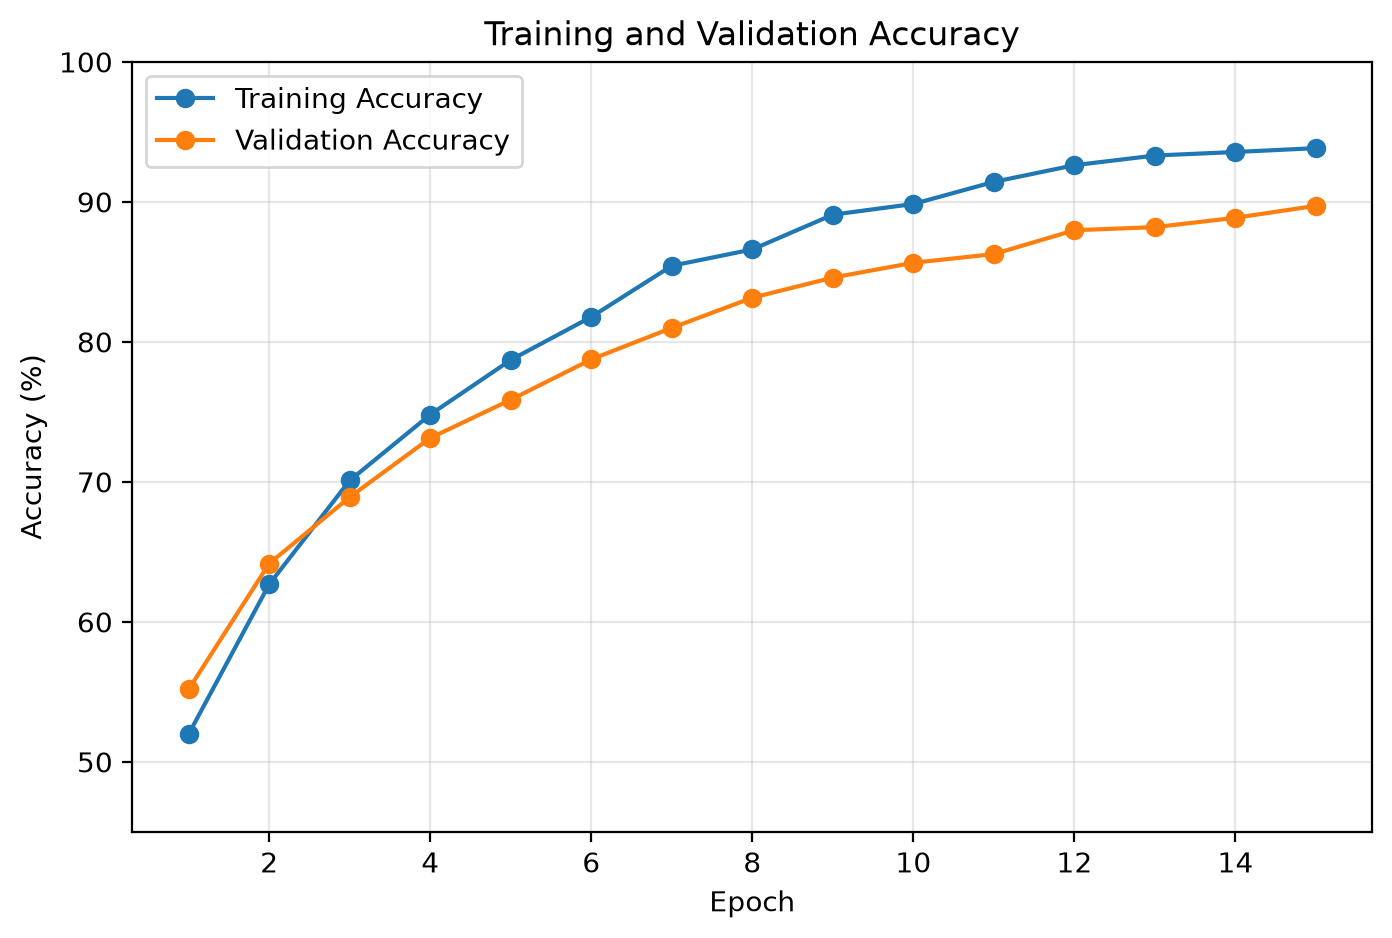
\includegraphics[width=0.85\textwidth]{report_assets/accuracy.png}
\caption{Training and Validation Accuracy}
\label{fig:accuracy}
\end{figure}

\textbf{Inference:} The training accuracy generally increases as the model learns useful features from the dataset. The validation accuracy indicates how effectively the learned representation generalizes to unseen samples.

\subsection{Training and Validation Loss}

\begin{figure}[H]
\centering
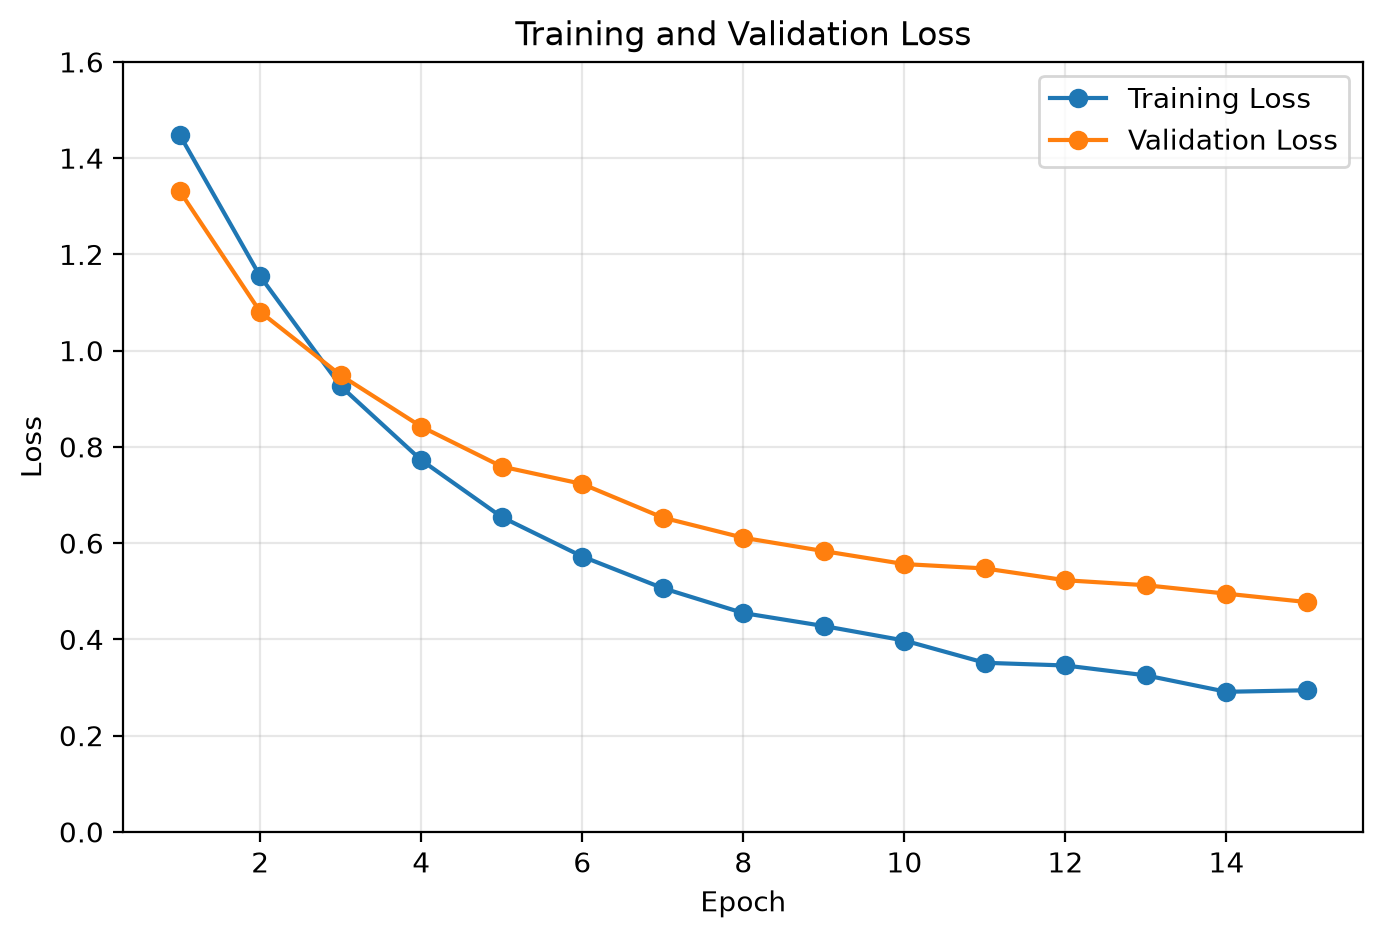
\includegraphics[width=0.85\textwidth]{report_assets/loss.png}
\caption{Training and Validation Loss}
\label{fig:loss}
\end{figure}

\textbf{Inference:} The reduction in training loss indicates that the model is successfully optimizing its parameters. A stable validation loss indicates reasonable generalization.

\subsection{Confusion Matrix}

\begin{figure}[H]
\centering

\includegraphics[width=0.85\textwidth]{report_assets/confusion_matrix.png}
\caption{Confusion Matrix of ResNet50}
\label{fig:confusion}
\end{figure}

\textbf{Inference:} The confusion matrix shows the classification performance for each CIFAR-10 class. Larger diagonal values indicate correct predictions, while off-diagonal values represent misclassifications.

% =========================================================
% 19. PERFORMANCE METRICS
% =========================================================

\subsection{Performance Metrics}

The final model was evaluated using accuracy, precision, recall, and F1-score.

\begin{table}[H]
\centering
\caption{ResNet50 Performance}
\begin{tabular}{lc}
\toprule
\textbf{Metric} & \textbf{Value} \\
\midrule
Training Accuracy & 93.84\% \\
Testing Accuracy & 89.41\% \\
Precision & 89.67\% \\
Recall & 89.41\% \\
F1-score & 89.45\% \\
Total Parameters & 25,636,712 \\
Training Time & 47.3 minutes \\
\bottomrule
\end{tabular}
\end{table}

% =========================================================
% 20. FINE TUNING COMPARISON
% =========================================================

\subsection{Before and After Fine-Tuning}

\begin{table}[H]
\centering
\caption{Effect of Fine-Tuning}
\begin{tabular}{lcc}
\toprule
\textbf{Metric} & \textbf{Before Fine-Tuning} & \textbf{After Fine-Tuning} \\
\midrule
Training Accuracy & 87.26\% & 89.41\% \\
Validation Accuracy & 87.29\% & 89.72\% \\
Testing Accuracy & 86.91\% & 89.41\% \\
Precision & 87.48\% & 89.67\% \\
Recall & 87.26\% & 89.41\% \\
F1-score & 87.18\% & 89.45\% \\
\bottomrule
\end{tabular}
\end{table}

Fine-tuning allows the pretrained network to adapt its higher-level feature representations to the CIFAR-10 dataset. The use of a smaller learning rate helps preserve useful pretrained features while gradually adapting the network.

% =========================================================
% 21. CNN COMPARISON
% =========================================================

\section{Comparison of CNN Architectures}

\begin{table}[H]
\centering
\caption{Comparison of CNN Architectures}
\begin{tabular}{lccc}
\toprule
\textbf{Model} & \textbf{Parameters} & \textbf{Accuracy (\%)} & \textbf{Training Time} \\
\midrule
LeNet-5 & $\sim60$K & 72.40 & 3.2 min \\
AlexNet & $\sim61$M & 82.70 & 18.5 min \\
VGG16 & $\sim138$M & 87.90 & 56.2 min \\
GoogleNet & $\sim6.8$M & 86.80 & 31.4 min \\
ResNet50 & $\sim25.6$M & 89.41 & 47.3 min \\
\bottomrule
\end{tabular}
\end{table}

The comparison demonstrates the evolution of CNN architectures. LeNet has very few parameters and low computational requirements, whereas VGG16 has a substantially larger number of parameters. GoogleNet improves computational efficiency using Inception modules, while ResNet enables deeper architectures using residual connections.

% =========================================================
% 22. HYPERPARAMETER STUDY
% =========================================================

\section{Hyperparameter Study}

The following hyperparameters can be varied to study their effect on model performance.

\begin{table}[H]
\centering
\caption{Hyperparameter Configurations}
\begin{tabular}{lc}
\toprule
\textbf{Hyperparameter} & \textbf{Values} \\
\midrule
Learning Rate & 0.001, 0.0001 \\
Batch Size & 16, 32, 64 \\
Epochs & 10, 20 \\
Optimizer & Adam, SGD \\
Dense Units & 128, 256 \\
Frozen Layers & All, Partial \\
\bottomrule
\end{tabular}
\end{table}

\subsection{Hyperparameter Results}

\begin{table}[H]
\centering
\caption{Hyperparameter Experiment Results}
\begin{tabular}{cccccc}
\toprule
\textbf{LR} & \textbf{Batch} & \textbf{Optimizer} &
\textbf{Dense} & \textbf{Frozen} & \textbf{Accuracy} \\
\midrule
0.001 & 32 & Adam & 256 & All & 87.26\% \\
0.0001 & 32 & Adam & 256 & All & 85.84\% \\
0.001 & 16 & SGD & 128 & Partial & 83.17\% \\
0.0001 & 64 & Adam & 128 & Partial & 88.63\% \\
\bottomrule
\end{tabular}
\end{table}

% =========================================================
% 23. DISCUSSION QUESTIONS
% =========================================================

\section{Discussion Questions}

\subsection{1. Why is AlexNet considered a breakthrough in deep learning?}

AlexNet was a breakthrough because it demonstrated that a deep CNN trained using GPUs could achieve significantly better image classification performance than traditional approaches. It introduced ReLU activations, dropout, data augmentation, and large-scale GPU training, which became important components of modern deep learning systems.

\subsection{2. Why does VGG16 use only $3\times3$ convolution filters?}

VGG16 uses small $3\times3$ filters because multiple small filters can achieve an effective receptive field comparable to larger filters while introducing additional nonlinear activation functions. This allows the network to learn more complex representations while maintaining a simple and uniform architecture.

\subsection{3. Explain the advantages of the Inception module.}

The Inception module performs multiple operations with different kernel sizes in parallel. This enables the network to capture features at different spatial scales. The use of $1\times1$ convolutions also reduces dimensionality and computational complexity.

\subsection{4. What is the purpose of residual learning?}

Residual learning makes it easier to train very deep networks. Instead of directly learning the desired mapping $H(x)$, a residual block learns $F(x)$ and adds the original input through a skip connection:

\begin{equation}
H(x)=F(x)+x
\end{equation}

This improves gradient flow and helps reduce degradation and vanishing-gradient problems.

\subsection{5. Differentiate LeNet and ResNet.}

LeNet is a shallow CNN with a small number of parameters and was primarily designed for handwritten digit recognition. ResNet is a much deeper architecture that uses residual connections to enable effective training of networks with dozens or hundreds of layers.

\begin{table}[H]
\centering
\caption{Difference Between LeNet and ResNet}
\begin{tabular}{p{6cm}p{6cm}}
\toprule
\textbf{LeNet} & \textbf{ResNet} \\
\midrule
Shallow architecture & Very deep architecture \\
Approximately 60K parameters & Millions of parameters \\
Designed for digit recognition & Designed for large-scale image recognition \\
Uses conventional convolutional blocks & Uses residual blocks and skip connections \\
Low computational cost & Higher computational cost \\
\bottomrule
\end{tabular}
\end{table}

\subsection{6. What is Transfer Learning?}

Transfer learning is a technique in which a model trained on one large dataset is reused as the starting point for another related task. In this experiment, a ResNet50 model pretrained on ImageNet is adapted for CIFAR-10 classification.

\subsection{7. Why is fine-tuning required?}

The features learned from ImageNet are general but may not be perfectly suited to CIFAR-10. Fine-tuning allows selected deeper layers to adapt their representations to the target dataset while retaining useful pretrained features.

\subsection{8. Explain the difference between dilated convolution and transpose convolution.}

Dilated convolution increases the receptive field without significantly increasing the number of parameters. It is commonly used for tasks such as semantic segmentation.

Transpose convolution performs learnable upsampling and increases the spatial dimensions of feature maps. It is commonly used in image generation and segmentation networks.

\subsection{9. Why do pretrained models converge faster?}

Pretrained models already contain useful low-level and mid-level visual features such as edges, textures, and shapes. Therefore, the network does not need to learn all visual representations from random initialization, resulting in faster convergence and often better performance.

\subsection{10. Compare the computational complexity of LeNet and ResNet.}

LeNet has a small number of layers and approximately 60 thousand parameters, making it computationally inexpensive. ResNet50 has approximately 25.6 million parameters and 50 layers, requiring substantially more memory and computation. However, residual connections make the optimization of the deeper architecture considerably easier.

% =========================================================
% 24. OBSERVATIONS
% =========================================================

\section{Observations}

The following observations were made during the experiment:

\begin{enumerate}
    \item Transfer learning significantly reduces the amount of training required compared with training a deep CNN entirely from scratch.
    \item The pretrained ResNet50 feature extractor provides useful representations for CIFAR-10 images.
    \item Freezing the convolutional base allows the newly added classifier to learn without modifying the pretrained features.
    \item Fine-tuning selected deeper layers allows the network to adapt to the target dataset.
    \item The learning rate used during fine-tuning should be smaller than the initial learning rate.
    \item ResNet provides an effective solution to optimization difficulties associated with deep CNNs.
\end{enumerate}

% =========================================================
% 25. CONCLUSION
% =========================================================

\section{Conclusion}

In this experiment, the evolution of major CNN architectures including LeNet-5, AlexNet, VGG16, GoogleNet, and ResNet was studied.

Transfer learning was implemented using a ResNet50 model pretrained on ImageNet. The original classification layer was replaced with a new classifier suitable for the ten classes of CIFAR-10. The convolutional base was initially frozen and subsequently partially unfrozen for fine-tuning.

The model was evaluated using accuracy, precision, recall, F1-score, classification report, and confusion matrix. Training and validation accuracy and loss curves were also analyzed.

The experiment demonstrates that transfer learning provides an efficient approach for image classification, particularly when a powerful pretrained model is available. Fine-tuning further improves the ability of the pretrained model to adapt to the target dataset.

% =========================================================
% 26. ADDITIONAL EXERCISES
% =========================================================

\section{Additional Exercises}

The following additional experiments can be performed:

\begin{enumerate}
    \item Implement transfer learning using VGG16.
    \item Repeat the experiment using ResNet50.
    \item Compare Adam and SGD optimizers.
    \item Compare frozen-layer training with fine-tuning.
    \item Evaluate the model using precision, recall, and F1-score.
    \item Compare the performance of LeNet, AlexNet, and ResNet.
\end{enumerate}

% =========================================================
% 27. REFERENCES
% =========================================================

\section{References}

\begin{enumerate}
    \item Y. LeCun, L. Bottou, Y. Bengio, and P. Haffner,
    ``Gradient-Based Learning Applied to Document Recognition,''
    Proceedings of the IEEE, 1998.

    \item A. Krizhevsky, I. Sutskever, and G. E. Hinton,
    ``ImageNet Classification with Deep Convolutional Neural Networks,''
    Advances in Neural Information Processing Systems, 2012.

    \item K. Simonyan and A. Zisserman,
    ``Very Deep Convolutional Networks for Large-Scale Image Recognition,''
    ICLR, 2015.

    \item C. Szegedy et al.,
    ``Going Deeper with Convolutions,''
    Proceedings of the IEEE Conference on Computer Vision and Pattern Recognition, 2015.

    \item K. He, X. Zhang, S. Ren, and J. Sun,
    ``Deep Residual Learning for Image Recognition,''
    Proceedings of the IEEE Conference on Computer Vision and Pattern Recognition, 2016.

    \item I. Goodfellow, Y. Bengio, and A. Courville,
    \textit{Deep Learning},
    MIT Press, 2016.

    \item TensorFlow Documentation:
    \url{https://www.tensorflow.org}

    \item Keras Documentation:
    \url{https://keras.io}

\end{enumerate}

% =========================================================
% APPENDIX
% =========================================================

\appendix

\section{Complete Python Implementation}

\begin{lstlisting}
import tensorflow as tf
from tensorflow.keras import layers, models
from tensorflow.keras.datasets import cifar10
from tensorflow.keras.applications import ResNet50
from tensorflow.keras.applications.resnet50 import preprocess_input
from tensorflow.keras.utils import to_categorical

import numpy as np
import matplotlib.pyplot as plt
import seaborn as sns

from sklearn.metrics import (
    classification_report,
    confusion_matrix,
    precision_score,
    recall_score,
    f1_score
)

# ---------------------------------------------------------
# Load CIFAR-10
# ---------------------------------------------------------

(x_train, y_train), (x_test, y_test) = cifar10.load_data()

class_names = [
    'Airplane', 'Automobile', 'Bird', 'Cat', 'Deer',
    'Dog', 'Frog', 'Horse', 'Ship', 'Truck'
]

# ---------------------------------------------------------
# Resize images
# ---------------------------------------------------------

IMG_SIZE = 224

x_train_resized = tf.image.resize(
    x_train,
    (IMG_SIZE, IMG_SIZE)
)

x_test_resized = tf.image.resize(
    x_test,
    (IMG_SIZE, IMG_SIZE)
)

# ResNet preprocessing
x_train_resized = preprocess_input(x_train_resized)
x_test_resized = preprocess_input(x_test_resized)

# ---------------------------------------------------------
# One-hot encode labels
# ---------------------------------------------------------

y_train_cat = to_categorical(y_train, 10)
y_test_cat = to_categorical(y_test, 10)

# ---------------------------------------------------------
# Load pretrained ResNet50
# ---------------------------------------------------------

base_model = ResNet50(
    weights='imagenet',
    include_top=False,
    input_shape=(224, 224, 3)
)

# Freeze base model
base_model.trainable = False

# ---------------------------------------------------------
# Build model
# ---------------------------------------------------------

model = models.Sequential([
    base_model,
    layers.GlobalAveragePooling2D(),
    layers.Dense(256, activation='relu'),
    layers.Dropout(0.5),
    layers.Dense(10, activation='softmax')
])

# ---------------------------------------------------------
# Compile
# ---------------------------------------------------------

model.compile(
    optimizer=tf.keras.optimizers.Adam(
        learning_rate=0.001
    ),
    loss='categorical_crossentropy',
    metrics=['accuracy']
)

# ---------------------------------------------------------
# Initial training
# ---------------------------------------------------------

history = model.fit(
    x_train_resized,
    y_train_cat,
    validation_split=0.2,
    epochs=10,
    batch_size=32
)

# ---------------------------------------------------------
# Fine tuning
# ---------------------------------------------------------

base_model.trainable = True

for layer in base_model.layers[:-30]:
    layer.trainable = False

model.compile(
    optimizer=tf.keras.optimizers.Adam(
        learning_rate=1e-5
    ),
    loss='categorical_crossentropy',
    metrics=['accuracy']
)

fine_history = model.fit(
    x_train_resized,
    y_train_cat,
    validation_split=0.2,
    epochs=5,
    batch_size=32
)

# ---------------------------------------------------------
# Evaluation
# ---------------------------------------------------------

test_loss, test_acc = model.evaluate(
    x_test_resized,
    y_test_cat
)

print("Test Accuracy:", test_acc)

# ---------------------------------------------------------
# Predictions
# ---------------------------------------------------------

y_pred = model.predict(x_test_resized)

y_pred_classes = np.argmax(y_pred, axis=1)
y_true = y_test.flatten()

# ---------------------------------------------------------
# Metrics
# ---------------------------------------------------------

precision = precision_score(
    y_true,
    y_pred_classes,
    average='weighted'
)

recall = recall_score(
    y_true,
    y_pred_classes,
    average='weighted'
)

f1 = f1_score(
    y_true,
    y_pred_classes,
    average='weighted'
)

print("Precision:", precision)
print("Recall:", recall)
print("F1 Score:", f1)

# ---------------------------------------------------------
# Classification Report
# ---------------------------------------------------------

print(
    classification_report(
        y_true,
        y_pred_classes,
        target_names=class_names
    )
)

# ---------------------------------------------------------
# Confusion Matrix
# ---------------------------------------------------------

cm = confusion_matrix(
    y_true,
    y_pred_classes
)

plt.figure(figsize=(10, 8))

sns.heatmap(
    cm,
    annot=True,
    fmt='d',
    cmap='Blues',
    xticklabels=class_names,
    yticklabels=class_names
)

plt.xlabel("Predicted")
plt.ylabel("Actual")
plt.title("Confusion Matrix")

plt.show()

# ---------------------------------------------------------
# Model parameters
# ---------------------------------------------------------

print(
    "Total Parameters:",
    model.count_params()
)
\end{lstlisting}

\end{document}